\documentclass{article}
\usepackage[utf8]{inputenc}
\usepackage[english]{babel}
\usepackage{amsthm}
\usepackage{graphicx}
\usepackage{amssymb }
\usepackage{amsmath}
\theoremstyle{definition}
\newtheorem{definition}{Definition}[section]
\theoremstyle{remark}
\newtheorem*{remark}{\textbf{Remark}}
\usepackage{blindtext}
\usepackage{geometry}
 \geometry{
 a4paper,
 total={190mm,280mm},
 left=10mm,
 top=10mm,
 }
 \usepackage{tabularx}

\title{Teoria dei Giochi a pillole}
\begin{document}
\graphicspath{ {./images/} }
\begin{itemize}
    \item \textbf{Gioco}: Un gioco è una tripla \(\Gamma=\{N,\{X_i\}_{i\in N},\{C_i\}_{i\in N}:N=\{1,..,n\}\}\) Insieme dei giocatori;$X_i$ non vuoto insieme delle strategie del giocatore i; $C_i$ payoff in fomra di costo.
    \item \textbf{Stato}:Vettore $(x_1,..,x_n)$ con $x_i\in X_i\ \forall i$;
    \item \textbf{Strategia del giocatore $i$ sapendo la giocata di un altro giocatore}:$x_i=(x_1,..,x_{i-1},x_{i+1},..,x_n)$;
    \item \textbf{Payoff del giocatore $i$ sapendo la giocata di un altro giocatore}:$C_i(x_i,x_{-i})$;
    \item \textbf{Best Response}: $B_i(x_{-i})$ è l'insieme delle migliori strategie che il giocatore $i$ èuò utilizzare se gli altri giocatore giocano $x_{-i}$: $B_i(x_{-i})=\{x_i^{'}\in X_i:C_i(x_i^{'},x_{-i})\leq C_i(x_i,x_{-i})\}$;
    \item \textbf{Strategia debolmente dominante}: Una strategia $x_i^{'}\in X_i$ è debolmente dominante per il giocatore i se, per ogni punto ammissibile $(x_i,x_{-i})$ con $x_i \neq x_{i}^{'}$ risulta: $:C_i(x_i^{'},x_{-i})\leq C_i(x_i,x_{-i})\}$. Quindi se e solo se $x_i\in  B_i(x_{-i})$ appartiene alle best response;
    \item\textbf{Strategia strettamente dominante}: è una strategia debolmente dominante, ma con il segno della disequazione con il minore stretto;
    \item \textbf{Ottimo debole di Pareto}: Dato un gioco $\Gamma$, un punto ammissibile $x=(x_1,..,x_n)$ è un ottimo debole di Pareto se non esiste un punto ammissibile $x'$ tale che $C_i(x')<C_i(x) \forall i\in N$. Se un punto x è un ottimo debole secondo Pareto, vuol dire che anche se i giocatori considerasse altir punti, esiste sempre un giocatore che non ha interesse a spostarsi da x: non è un ottimo debole se entrambi i giocatori migliorano il payoff.
    \item \textbf{Ottimo forte secondo Pareto}: Dato un gioco $\Gamma$, un punto ammissibile $x=(x_1,..,x_n)$ è un ottimo forte di Pareto se non esiste un punto ammissibile $x'$ tale che  $C_i(x')<\leq C_i(x)$ per ogni giocatore e $C_h(x')<C_h(x)$ per almento un giocatore.
    \item \textbf{Strategia dominante e Ottimo Pareto}: se l'incrocio delle strategie dominante è un punto di ottimo debole di pareto, allora questa sarà la soluzione probabile del gioco.
    \item \textbf{Equilibrio di Nash}: Dato un gioco $\Gamma$ e un suo punto ammissibile, esso è un equilibrio di Nash per il gioco se risulta per ogni giocatore:$C_i(x_i*,x_{-i}*)\leq C_i(x_i,x_{-i}*)\ \forall x_i\in X_i$.\newline Un punto è un equilibrio di Nash per il gioco se e solo se $x_i*\in B_i(x_{-i}*)$ ogni strategia appartiene alla best response.\newline Un punto è un equilibrio di Nash se nessun giocatore può migliorare il proprio payoff modificando in modo unilaterale la propria strategia;
    \item \textbf{Pollution Game}:\begin{itemize}
        \item \textbf{Gioco:} Estensione del dilemma dei prigionieri sul controllo delle emissioni e sull'inquinamento: se il giocatore i inquina aggiunge una unità di costo al payoff di ciascun giocatore.
        \item \textbf{Svolgimento:}\begin{enumerate}
        \item \textbf{Formalizzazione}: \(x_i=1\) se il giocatore i controlla le emissioni e \(x_i=0\) se il giocatore i sceglie di inquinare.
            \item Consideriamo un qualunque stato in cui almeno un giocatore controlla le emissioni.
            \item Il suo payoff sarà pari a \(C_i(x_i)=3x_i+\sum_{j=1,\dots,n}(1-x_j)\);
            \item Si osserva che \(C-i(x_i,x_{x_i})=2x_i+n-t\quad t=\sum_{j\neq i}x_j\);
            \item \textbf{Equilibrio di Nash}: L'unico equilibrio di Nash è \(0,\dots,0\), ma non è stabile;
        \end{enumerate}
    \end{itemize}
    \item \textbf{Strategie Dominanti e E.N.}: Se ogni giocatore ha una strategia debolmente dominante, allora il punto di incrocio di queste strategie è un equilibrio di Nash.\newline Se ogni giocatore ha una strategia strettamente dominante allora il punto di incrocio è l'unico equilibrio di Nash del gioco.
    \item \textbf{Strategia Conservativa}: Una strategia è detta minimax/conservativa per il giocatore i se risulta:$\tilde{C}_i(x_i)=min_{x_{i}\in X_{i}}C_i(x_i)$. Equivale a minimizzare quello che si dovrà pagare nel caso peggiore.
    \item \textbf{Stratergia Dominante e Conservativa}: Se per un giocatore i esiste una strategia debolmente dominante, allora è anche una strategia conservativa per il giocatore.
    \item \textbf{Equilibri di Nash e Giochi Antagonistici};\begin{itemize}
        \item \textbf{Gioco a somma costante}: Un gioco è a somma costante se per stato del gioco risulta che la sommatoria dei payoff è costante. Viene detto a somma zero se la somma è zero.
        \item \textbf{Gioco Antagonistico} Un gioco a somma zero con due giocatori è detto antagonistico se per ogni stato del gioco risulta il payoff del primo giocatore uguale a - payoff del secondo giocatore.
        \item \textbf{Gioco Simmetrico}: un gioco antagonistico è detto simmetrico se la matrice dei payoff è antisimmetrica.
        \item \textbf{Equilibrio di Nash Gioco Antagonista}: Uno stato di un gioco antagonisa è di Nash se: $C(x_1,x_2*)\geq C(x_1*,x_2*)\forall x_1\in X_1,\forall x_2\in X_2$;
        \item \textbf{Gioco Antagonista con funzioni}:\begin{itemize}
            \item \textbf{Equilibrio di Nash}: Un equilibrio di Nash è un punto di sella della funzione di Payoff.
            \item \textbf{Strategia Conservativa}:
            \begin{center}
                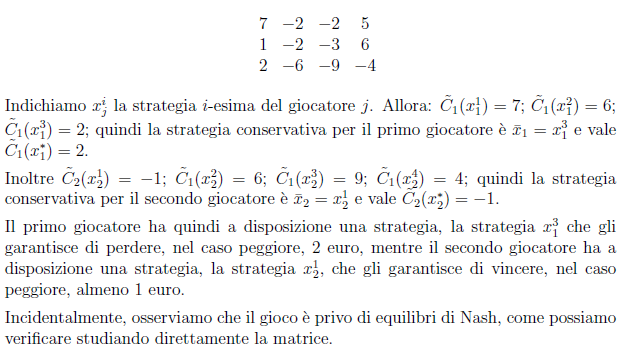
\includegraphics[scale=0.7]{image100.png}
            \end{center}
            \item \textbf{Equilibrio di Nash}: Per un gioco antagonista un punto ammissibile è un equilibrio di Nash se e solo se le strategie del primo e seconod giocatore sono strategie conservative per i corrispettivi giocatori.
        \end{itemize}
        \item \textbf{Valore di un gioco Antagonista}: Il valore delle strategie consrvative dell'equilibrio di Nash è detto valore del gioco antagonista.\newline Un gioco a valore zero è detto fair e nel caso di un gioco simmetrico esso è sempre 0.
        \item \textbf{Giochi Antagonistici infiniti}: In questa casistica non sempre esiste una strategia conservativa. Nel caso in qui esistesse, allora valgono le considerazioni del caso finito: il gioco ha un equilibrio di Nash se e solo se le rispettive straegie sono conservative.
        \item \textbf{Giochi Strettamente Competitivi}: Un gioco con due giocatori è strettamente competitivo se vale: $C_1(x^a)\leq C_1(x^b)$ se e solo se $C_2(x^a)\geq C_2(x^b)\ \forall x^a,x^b$
    \end{itemize}
    \item \textbf{Equilibri di Nash in Strategia Mista}:\begin{itemize}
        \item \textbf{Estensione in strategia mista}: Dato un gioco finito in forma normale, l'estensione in strategia mista è un nuovo gioco infinito definito da:\begin{center}
            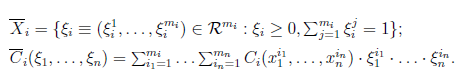
\includegraphics[scale=0.6]{images/image99.png}
        \end{center}
        \item\textbf{Equilibrio di Nash}: In estensione in strategia mista di un gioco antagionista si ha un equilibrio di Nash se esiste una strategia conservativa per il primo e secondo giocatore e se e solo se: $C_1(x_11)=-C_2(x_2)$;
        \item \textbf{Strategie Conservative}: In estensione in strategia mista esistono sempre strategie conservative.
        \item \textbf{Problema PL}:Primo giocatore:\begin{center}
            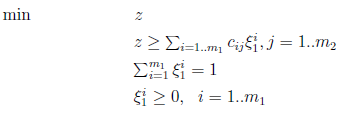
\includegraphics[scale=0.6]{images/image98.png}
        \end{center}
        Secondo giocatore:\begin{center}
            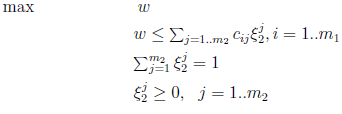
\includegraphics[scale=0.6]{images/image97.png}
        \end{center}
        \item \textbf{Equilibrio di Nash}: si ha ottimalita se w e z sono uguali. Questo punto sarà l'equilibrio di Nash. Questo equilibrio esiste sempre.
    \end{itemize}
    \item \textbf{Giochi Cooperativi}:\begin{itemize}
        \item \textbf{Gioco Cooperativo}:è un gioco in cui gruppi di giocatori possono coalizzarsi e garantire alla coalizione di una certà utilità.
        \item \textbf{Utilità trasferibile}: Un gioco cooperativo con utilità trasferibile è definit da una coppia $(N,v)$: N è l'insieme dei giocatori, $v$ è una funzione che associa ad ogni sottoinsieme S di N un utilità $v(S)$ tale che $v(insiemevuoto)=0$. Ciascun giocatore di S è detto coalizione e l'insieme N di tutti i giocatore è la grande coalizione.\newline L'utilità è trasferibile poiché per ogni coalizione l'utilità e definita in maniera cumulativa.
        \item \textbf{Grande Coalizione Stabile}: Ogni volta che esiste una soluzione che ripartisca tra tutti i giocatori l'utilità $v(N)$ della grande coalizione in modo tale che nessuna coalizione sia tentat dal rompere la grande colizione. Quinid esiste una soluzione $\alpha\in\mathbf{R^n}$ tale che:\begin{itemize}
            \item $\sum_{i\in S}\alpha_i\geq v(s)\quad\forall S in N$
            \item $\sum_{i\in N}\alpha_i=v(N)$;
            In cui $\alpha_i$ è il payoff assegnato dalla soluzione $\alpha$ al giocatore i
        \end{itemize}
        \item\textbf{Nucleo}: Il nucle è l'insieme dei vettori $\alpha\in\mathbf{R}_{+}^{n}$ tali che:\begin{itemize}
            \item $\sum_{i\in S}\alpha_i\geq v(s)\quad\forall S in N$
            \item $\sum_{i\in N}\alpha_i=v(N)$;
            In cui $\alpha_i$ è il payoff assegnato dalla soluzione $\alpha$ al giocatore i
        \end{itemize}
        \item\textbf{Stabilità}: La grande coalizione è stabile se il nuclo non è vuoto.
        \item\textbf{SuperAdditività}: Sia N un insieme. Indichiamo con $2^N$ la famiglia di tutti i sottoinsiemi di N. Una funzione $v:2^N$ è detta super additiva se soddisfa le seguenti proprietà:$v(S)+v(T)\leq v(S\cup T)\quad\forall S,T\subset N:S\cap T=\varnothing$
        \item\textbf{C.N.S. Superadditiva}: Una funzione $v$ è super additiva se e solo se:\begin{itemize}
            \item $v(\varnothing)=0$
            \item $\sum_{i=1..h}v(S_i)\leq v(Q) \forall Q \subseteq N$ e partizioni in classi $S_1,..S_h$
        \end{itemize}
        \item \textbf{Imputazione}: Un'imputazione per un gioco cooperativo $(N,v)$ è un vettore $\alpha$ che soddisfa le seguenti proprietà:\begin{center}
            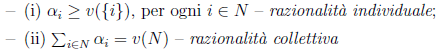
\includegraphics[scale=0.6]{images/image96.png}
        \end{center} Quindi è una soluzione del gioco che ripartisce tra i giocatori l'utilità della grande coalizione in modo tale che nessun giocatore singolo sia tenato dall'abbandonare la grande coalizione.L'insieme delle imputazioni è sempre non vuoto.
        \item\textbf{Giochi Inessenziali}: In un gioco cooperativo queste tre affermazioni sono equivalenti e caratterizzano i giochi inessenziali:\begin{center}
            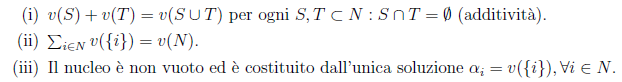
\includegraphics[scale=0.6]{images/image95.png}
        \end{center}
        \item\textbf{Soluzione Giochi Inessenziali}: Un gioco inessenziale ha come unica soluzione $\alpha_i=v(\{i\})\quad i\forall N$
        \item \textbf{Lemma} Il nucleo è non vuoto se e solo se il seguente problema di PL ha una soluzione ottima con valore $\leq v(N)$: \begin{center}
            $\sum \alpha_i$\newline
            $\sum_{i\in S}\alpha_i\geq v(S)\quad \forall S \in N_p$
        \end{center}
        Il suo problema duale è:\begin{center}
            $max \sum\lambda_sv(s)$\newline
            $\sum_{S\in N_{p:i\in S}}\lambda_s=1\quad i \in N$\newline $\lambda\geq0$
        \end{center}
        \item \textbf{Vettore bilanciato}: Un vettore $\lambda$ è detto bilanciato se per ogni $i\in N$ vale $\sum_{S\in N_{p:i\in S}}\lambda_s=1$.
        \item\textbf{Bondareva-Shaplet} Un gioco cooperativo ha nucleo non vuoto se e solo se è bilanciato.
    \end{itemize} 
    \item \textbf{Valore di Shapley}:\begin{itemize}
    \item \textbf{Importante:} Non è possibile calcolare il valore di Shapley se la somma della coalizione per rendere effettiva una legge è minore di \(\frac{N}{2}\)
        \item \textbf{Premessa}: Sia P l'insieme di tutte le permutazione dell'insieme N dei giocatori. presa una permutazione $p\in P$ e un giocatore $i\in N$ indichiamo con $A_i^p$ è la coalzione formata da i e da tutti i giocatori che precedono $i$ nella permutazione $p$.
        \item\textbf{Funzione payoff}: Consideriamo un gioco cooperativo $(N,v)$. La funzione che assegna a ciascun giocatore un payoff $S_i(v)$ deve soddisfare i seguenti assiomi:\begin{itemize}
            \item Assioma di razionalità collettiva: $\sum_{i\in N}=v(N)$;
            \item Sia $i\in N$. Se per ogni $T\subseteq N$ risulta $v(T\cup \{i\})=v(T)$;
            \item Siano $i,j\in N\neq j$. Se per ogni $T\subseteq N:i,j\not\in T$ risulta $v(T\cup\{i\})=v(T\cup\{j\})$ allora $S_i(v)=S_j(v)$;
            \item Sia u e v due funzipni di utilità. Allora $S(u+v)=S(u)+S(v)$.
        \end{itemize}
        \item \textbf{Teorema di Shapley}: Fissato un insieme N di giocatori, esiste una e una sola funzione S che soddisfa gli assiomi:\begin{center}
            $S_i(v)=\sum_{p\in P} \frac{1}{n!}(v(A_i^p)-v(A_i^p\backslash\{i\}))$
        \end{center}
        e $S(v)$ è una imputazione
        \item \textbf{Utilità Marginale}: è l'utilità che apporta il giocatore $i$ a $T$ ed è pari a $v(T)-v(T\backslash\{i\})$\newline Considerando tutte le permutazioni P dell'insieme N dei giocatori, si dice che l'utilità marginale apportata da i alla permutazione $p\in P$ è pari a $v(A_i^p)-v(A_i^p\backslash\{i\})$. Preso il valor medio dell'utilità marginale apportata da i a ciascuna permutazione di P si ottiene il valore $S_i(v)$
        \item \textbf{Alternative}:\begin{itemize}
            \item $S_i(v)=\sum_{T\subseteq N:i\in T}\frac{(|T|-1)!(n-|T|)!}{n!}(v(T)-v(T\backslash\{i\}))$
        \end{itemize}
        \item 1\textbf{Gioco Semplice}: Un gioco cooperativo è detto semplice se la funzione di utilità ha valore 0,1. Una coalizione in grado di imporre una decisione ha valore 1.\begin{center}
            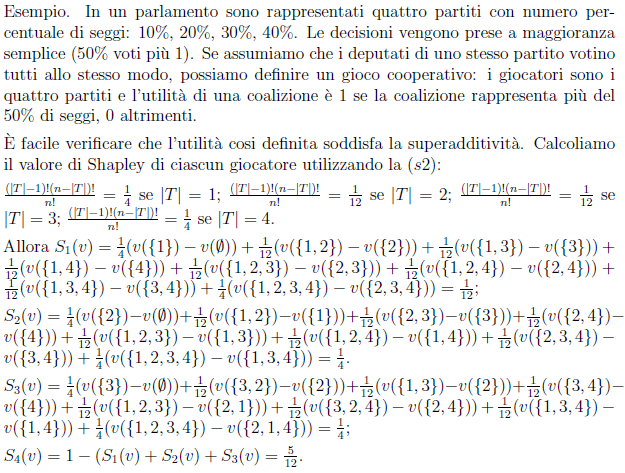
\includegraphics[scale=0.7]{images/image94.png}
        \end{center}
        \item\textbf{Valore Shapley Giochi Semplici}:\begin{itemize}
            \item $S_i(v)=\sum_{T\subseteq N: T\ vincente,\ T(i) perdente}\frac{(|T|-1)!(n-|T|)!}{n!}\quad\forall i\in N$
            \item $S_i(v)=\frac{1}{n!}\quad \forall i\in N$
        \end{itemize}
        \item \textbf{House Allocation Problem}: \begin{itemize}
            \item \textbf{Gioco}: Dato un insieme di n giocatori e un incieme C di n case. Ogni giocatore possiede una e una sola delle case; inoltre ogni giocatore ha in mente una graduatoria di tutte le n case
             dell'insieme C: ogni giocatore i, per ogni coppia di case \(u,v\in C\) preferusce u a v oppure v a u. L'obbiettivo è quello di riallocare le case tra i giocatori, ovvero trovare un matchin M di dimensione N che sia stabile.
             \item \textbf{Definizioni}: Per ogni insieme S di giocari definiamo \(V(S)\) come un qualunque matching che assegna a ciascun giocatore di S una e una sola casa dell'insieme C.
             \item \textbf{Obiettivo:}Vogliamo un matching \(M\in V(N)\) che assegna a ciasun giocatore di N una e una sola casa di C in modo tale che per ogni giocatore \(i\in S\), il matching M' assegna ad i una casa non peggiore di quella che
             gli assegna il matching M e per almento un giocatore \(j\in S\), il matching M' assegna a j una casa migliore di quella che gli assegna il matching M.\textbf{Stabilità}.
             \item \textbf{Agoritmo Top Trading Cycle TTCA}: \begin{itemize}
                 \item \textbf{Grafo:} Costruiamo una grafo orientato G: i nodi di G corrispondono ai giocatori di N e ogni nodo ha esattamente un successore corrispondente al proprietario che i preferisce tra quelle dell'insieme N.
                 L'unico arco usente da i è l'arco (i,i)m se la casa preferita da i è quella che possiede:\textbf{Loop}.\newline
                 G possiede per costruzione n nodi e n archi.
                 \item \textbf{Primo Matching}: In questo grafo possiamo sempre trovare dei cicli. Possiamo trovare un primo matchin parziale indotto dai cicli di G:\newline
                 Sia \(N_1\) l'insieme dei nodi appartenenti ad un ciclo di G, assegniamo a ogni giocare \(i\in N_1\) la casa posseduta al giocare \(j\in N_1\) tale che \((i,j)\in E(G)\) e rimuoviamo dal gioco i giocare di \(N_1\) con le corrispondenti case.
                 \item\textbf{Secondo Grafo:} Costruiamo un nuovo grafo \(G_1\) in cui l'insieme dei giocatori è \(N\backslash N_1\) e nuovamente ogni nodo i ha un unico successore corrispondente al proprietario della casa che i preferisce dtra quelle del nuovo insieme.\newline
                 A questo punto ragioniamo compre prima  e rimoniamo le case e i nodi corrispondeti ai nuovi cicli rispettando le preferenze dei ndodi.
                 \item\textbf{Termine:} In \(k\leq n\) l'algoritmo termina restituendo il matching.
                 \item  \textbf{Considerazioni}: L'algoritmo TTCA restituisce l'unico matching nel nucleo del gioco. Inoltre, se M non fosse stabile, esiste un nuovo matching e un giocare i che assegna ad i una casa migliore di quella assegnatagli dal matching ottimo.
             \end{itemize}
        \end{itemize}
        \item \textbf{Stable Marriage Problem:}\begin{itemize}
            \item \textbf{Gioco:} Sono dati 2n giocatori: n uomini ed n donne. Ogni giocare ha in mente una graduatoria di tutte le n persone dell'altro sesso. L'obiettivo è quello di accoppiare gli uomini con le n donne e quindi trovare
            un matchin M di dimensione n che sia stabile. Assumiamo che ogni giocatore preferisce in ogni caso accoppiarsi piuttosto che rimanere single.
            \item\textbf{Stabilità Matching}: Un matchin M di dimensione n è stabile se non esiste un insieme S di \(h\leq n\) uomini e h donne e un matching M' tra gli uomini e le donne di S tale che:\begin{itemize}
                \item Per ogni giocatore \(i\in S\), il matchin M' assegna a i un partner non peggiore, secondo le preferenze, di quella che aasegna il matchin M;
                \item Per almento un giocatore \(j\in S\) il matchin M' assegna a j un partner migliore dii quello che gli assegna il matchin M;
            \end{itemize}
            In particolare, \textbf{un matching M di dimensione n è stabile se e solo se non esistono un uomo me  una donna w tali che m preferisce w al partner che il matchin gli assegna, e w preferisce m al partner che gli assegna il matching.}
            \item\textbf{Algoritmo di Gale-Shapley}:\begin{itemize}
                \item \textbf{Prima Iterazione:} Alla prima iterazione ogni uomo si propone alla donna che preferisce. Ogni donna considera tutte le proposte che ha ricevuto e dice:
                    \textbf{FORSE}: all'uomo che prescerisce tra quelli che le si sono proposti,
                    \textbf{NO}: a tutti gli altri uomini che le si sono proposti.
                Le donne che hanno ricevuto una proposta a cui hanno risposto "Forse" sono temporaneamente fidanzate.
                \item\textbf{Iterazioni successive:}Ogni uomo non fidanzato si propone alla donna che preferisce, tra quello che non lo hanno già rifiutato. La donna esamina tutte le proposte
                fino ad ora ricevute e risponde con \textbf{FORSE} all'uomo che preferisce e \textbf{NO} a tutti gli altri. Ciò vuol dire che la donna può cambiare fidanzato e un uomo non può essere mollato.
                \item \textbf{Conslusione:} Si itera fino a quando tutte le donne sono temporaneamente fidanzate. Questi fidanzamenti sono il matching finale M proposto dall'algoritmo. Si termina in \(n^2\) iterazioni
                Ad ogni iterazione, tranne quella finale, almeno un uomo viene rifiutato: cancella la donna che lo ha rifiutato dalla sua graduatoria.
                \item\textbf{Considerazioni:}
                \begin{enumerate}
                    \item \textbf{Il Matching è stabile.}
                    \item Se una donna è temporaneamente fidanzata a una certa iterazione, lo sarà anche nell'iterazione successiva e con un uomo non peggiore in graduatoria.
                \end{enumerate}
                \item\textbf{Variante:} Se nell'algoritmo di Gale-Shapley avessero scelto le donne, avremmo identificato un diverso matching stabile.
            \end{itemize}
        \end{itemize}
        \item \textbf{Mercati Utilità trasferibile}:\begin{itemize}
            \item \textbf{Gioco}:Ci sono n agenti in grado di produrre un certo bene. Per produrre questo bene,ogni agente dispone di un insieme di risorse l che può utilizzare per produrre il bene e ha una propria funzione di
            produzione che restituisce la quaantità di bene che l'agente è in grado di produrre a partire dal vettore di risorse \(w_i\).
            In maniera formale, ogni agente dispone di un vettore di risorse \(w_i=(w_i^1,\dots,w_i^l)\in \\mathbf{R_+}\) e ha una sua funzione di produzione \(f_i\) ch associa al suo input \(w_i\) una quantità prodotta \(f(w_i)\) del bene.
            In questo mercato, gli agenti posso essere interessati a cooperare: se i vettori di risorse sono complementari, può essere utile scambiarsi delle risorse e si vuole massimizzare l'utilità che trarrà dalla produzione del bene.
            \item\textbf{Modellazione:}Il gioco viene modellato come gioco cooperativo: l'insieme dei giocatori coincide con quello degli agenti. Supponiamo che la coalizione S possa allocare in qualcunque modo tra gli agenti in S le risorse complessi
            vamente disponbili: \(w(S)=\sum_{i\in S}w_i\)
            \item\textbf{Svolgimento:} Il problema deve essere formulato in termini di problema di ottimizzazione. Indichiamo con \(z_i\in R\) il vettore delle risorse assegnato all'agente i con il corrispondente \textbf{vincolo di ammissibilità}:\(\\sum_{i\in S}^{}z_i=\sum_{i\in S}w_i\).\newline
            Occorre quindi risolvere il problema:
            \begin{equation}
                v(S)=max \sum_{i\in S}f_i(z_i)
            \end{equation}
            \begin{equation}
                \sum_{i\in S}z_i=\sum_{i\in S}w_i
            \end{equation}
            \begin{equation}
                z_i\geq 0
            \end{equation}
            Questo problema ha sempre soluzione dato che la funzione obiettivo è continua su insieme chiuso e limitato.
            \item \textbf{Funzione di utilità}: la funzione di utilità è \textbf{Superadditiva}.
            \item Ogni mercato con utilità trasferibile ha un nucleo non vuoto.
        \end{itemize}
    \end{itemize}
\end{itemize}
\newpage
\begin{center}
    \textbf{-ESERCIZI-}
\end{center}
\textbf{Strategia Mista:}\newline
\begin{center}
    \includegraphics*[scale=0.6]{2021-11-29-14-12-59.png}
\end{center}
1) Per ciascuna di queste strategie, indica quanto paga, nel caso peggiore, chi la usa.\newline
\begin{center}
    \begin{tabular}{|c |c |c |c |c |c |c |c |c |c |c | c|} 
     \hline
     \(\xi _1^1\) & \(\xi_1^2\) & \(\xi_1^3\) & \(\xi_1^4\) & z & max z & \(\xi_2^1\) & \(\xi_2^2\) & \(\xi_2^3\) & \(\xi_2^4\) & -z & max z\\ [0.5ex] 
     \hline
      & & & & & & & & & & &\\
     \hline
     \\
     \hline
     \\
     \hline
     \\
     \hline
     \\
     \hline
     \\ [1ex] 

    \end{tabular}
    \end{center}
\end{document}